\documentclass[12pt, oneside]{article}   	% use "amsart" instead of "article" for AMSLaTeX format
\usepackage{textcomp}
\usepackage{geometry}                		% See geometry.pdf to learn the layout options. There are lots.
\geometry{letterpaper}                   		% ... or a4paper or a5paper or ... 
%\geometry{landscape}                		% Activate for rotated page geometry
%\usepackage[parfill]{parskip}    		% Activate to begin paragraphs with an empty line rather than an indent
\usepackage{graphicx}				% Use pdf, png, jpg, or eps§ with pdflatex; use eps in DVI mode
\usepackage{caption}
\usepackage{subcaption}								% TeX will automatically convert eps --> pdf in pdflatex		
\usepackage{hyperref}
\usepackage{amssymb}
\usepackage{amsthm}
\newtheorem{theorem}{Theorem}
\newtheorem{definition}{Definition}
\usepackage{natbib}
\usepackage{xcolor}
\usepackage{hyperref}
\usepackage{authblk}
\hypersetup{
    colorlinks=false,
    linkcolor=blue,
    filecolor=magenta,      
    urlcolor=blue,
    pdfpagemode=FullScreen,
}
\usepackage{float}
\usepackage{rotating}
\usepackage{adjustbox}
\usepackage[font=small,labelfont=bf]{caption}

\usepackage{authblk}
\title{Detecting Overlapping Research Communities}
\author[1]{Akhil Jakatdar}
\author[1]{Tandy Warnow\thanks{warnow@illinois.edu}}
\author[1,2]{George Chacko\thanks{chackoge@illinois.edu}}
\affil[1]{Department of Computer Science, University of Illinois Urbana-Champaign, Urbana, IL 61801}
\affil[2]{Office of Research, Grainger College of Engineering, University of Illinois Urbana-Champaign, Urbana, IL 61801}

% \setlength{\parindent}{0pt}
%SetFonts

\begin{document}
\maketitle

\abstract{Community detection methods assist the understanding of complex networks through discovery of meso-scale structures. A variety of approaches have been developed for this purpose. However, many community finding methods rely on disjoint clustering techniques, in which a node is only assigned to one community or cluster. This strict requirement limits the ability to inclusively describe communities since some nodes may reasonably be assigned to many communities. Whereas we previously reported a scalable and modular pipeline that discovers disjoint research communities from the scientific literature, we now present an enhancement in the for of a complementary overlapping community approach.  We present findings from this new approach on a network of over 13.99 million nodes that captures recent research in the very rapidly growing field of extracellular vesicle research.}

\clearpage

\section{Introduction} Research communities represent scientific specialization \citep{Chubin1976,Morris2009} that evolves in response to influences such as new research paradigms, policy effects, collaboration practices, increasing globalization, and large-scale reorganization. The problem of identifying and characterizing research communities in the modern scientific enterprise motivates the work presented in this article. We are interested in scalable methods for identifying research communities as they emerge and grow to maturity. We would also like to understand the extent to which these communities overlap. 

Beyond identifying communities, we are interested in their structure and roles played by community members. Of special interest is the core-periphery or center-periphery structure \citep{Breiger2014} since \cite{Price1966}, in their study of the oxidative phosphorylation community reported center-periphery structure: a small core of influential researchers and a much larger transient population. Core-periphery or center-periphery patterns have also been reported in other networks using different techniques, such as block modeling and k-core decomposition, arguing for some degree of ubiquity in their occurrence \citep{borgatti2000models,Rombach2017,gallagher2021clarified,yanchenko_2202.04455}. 

%Tandy - come back to this paragraph
A considerable literature exists on community finding in graphs that reflects a diversity of perspectives and solutions. These diverse approaches can be drawn upon in identifying research communities \citep{Fortunato2009,FORTUNATO201075,Coscia2011,Yang2016}.  Community finding and clustering approaches have been applied to the scientific literature~\citep{Newman2006,Fortunato2009,Boyack2010,Boyack2019,Traag2019,Ahlgren2020,Chandrasekharan2021,Wedell2022}. The majority of these approaches focus on disjoint partitioning, where a vertex or node is only assigned to only one community. 
This is a limitation when analyzing citation data, since some nodes can reasonably be assigned to more than one community; for example, publications introducing widely used methods may be integral to the research activities of multiple communities. 
Several methods have been developed that can produce overlapping clusters \citep{Baumes2005,Palla2005,banerjee2005model,Cleuziou2008,Lancichinetti2009,Lu2012}, although they do not appear to enjoy wide use in scientometric studies. 

One approach to identifying research communities is through analyzing citation patterns in the scientific literature. The underlying assumption is that members of a research community are more likely to cite each other's work than the work from outside their community.  Drawing upon the rich literature on graph theory, this question can then be framed as a community finding problem where a community is defined as a set of vertices in a graph that exhibit stronger connectivity to each other than to vertices outside such a community. Thus, in the graph (or network) of scientific literature, citation-dense areas suggest the existence of communities of publications. This approach is different from characterizing the publications authored by members of known communities \citep{Price1966,crane1972invisible,smallspecialties1979,Mullins1985} since the community is first defined by edge-density and then 
its members are inferred from the authors of the community of publications \citep{Chandrasekharan2021,Wedell2022}.

We stress that citation density alone does not make a confirming argument for the existence of a community. However, community finding techniques are valuable in being able to search large datasets for communities, efficiently reducing them to smaller data that can then be examined with complementary techniques that include the use of domain expertise.

We recently reported Iterative K-core Clustering or IKC \citep{Wedell2022}, a recursive algorithmic approach based on the k-core property \citep{Giatsidis2011,malliaros2019}, which helps identify densely connected parts of a graph. IKC recursively extracts disjoint k-cores from a graph beginning with the most dense  k-core and until some user-specified value of $k$ is reached. IKC avoids global modularity maximization \citep{lancichinetti2011limits} but enforces positive modularity for individual communities and the minimum value of $k$ set by a user. 

We implemented IKC as the first step in a tunable modular pipeline to identify communities with core-periphery structure. Subsequent steps in the pipeline include breaking large cores, and adding peripheral nodes to each core to construct communities with core-periphery structure. While IKC is a necessary step in the pipeline, the remaining steps are optional. We tested this pipeline against a network of greater than 14 million articles that are centered around the rapidly growing field of extracellular vesicle (EV) biology \citep{Wedell2022}. Using the IKC pipeline, we were able to identify two communities of interest, rich in EV literature, that were robust to various option settings \citep[Figures 5]{Wedell2022}, effectively reducing a very large dataset to foci of interest. 

However, IKC produces disjoint clusters, and some articles can reasonably be assigned to more than one community. 
As noted above, this limitation impacts articles that describe widely used methods but is also relevant, in theory at least, to articles reporting discovery that are influential in more than one community.  Thus, a need for exists for methods that can produce meaningful overlapping clusters. 

Several methods have been developed that can produce overlapping clusters, although none of them were specifically designed to address core-periphery structure in the scientific literature  \citep{Baumes2005,Palla2005,banerjee2005model,Cleuziou2008,Lancichinetti2009,Lu2012}. An interesting approach is the two-step procedure where the input graph is first transformed into a line graph whose nodes represent edges in the original graph \citep{Harary1960}.  The line graph is then clustered and this output can be mapped back to the input graph to generate overlapping clusters. This general approach has been used by others on citation data \citep{Evans2009,Havemann2021}. However, line graph  techniques are not very scalable, since the size of a line graph is much larger than the size of its input graph. For example, the network that we studied in \cite{Wedell2022} would grow from 13,989,436 nodes and 92,051,051 edges to 92,051,051 nodes and 160,428,881,121 edges (Supplementary Materials), which presents a challenge to clustering software.
 
To address the limitation to disjoint clusters with IKC, we developed  ``Allowing Overlapping Clusters" (AOC), a scalable meta-method that takes the output of IKC and makes multiple community assignments from a list of candidate nodes. AOC can be used as an optional step in the IKC pipeline at the discretion of the user. We present results from AOC applied to the cores generated by the IKC method, and discuss the results and discovery made from them. 

While the overarching question that motivates our work is identifying and describing research communities, this article is focused on the more narrow question of extending the IKC method towards inclusively identifying the cores of core-periphery structured communities and towards more general use in community detection. We present results from testing this method on a network centered around the recent EV literature, a very rapidly growing field in biology \citep{van2022challenges}. 
 
\section{Materials and Methods}

\subsection{Methods} Motivated by the graph-theoretic concept of k-cores \citep{Giatsidis2011,malliaros2019}, we have previously constructed a clustering pipeline we refer to as  the Iterative K-core Clustering (IKC) pipeline in \cite{Wedell2022}, This scalable and tunable method takes, as input, two parameters $k$ and $p$ with $k > p \geq 1$, and computes a clustering of a given network $N$ into disjoint clusters where each cluster has a ``core'' component, and a ``periphery". This clustering is designed to satisfy several criteria: (1) the core of each cluster is connected,  has positive modularity ($m$-valid), and each node in the center  is adjacent to at least $k$ other nodes in the center ($k$-valid), and (ii) every node in the periphery of a cluster is adjacent to at least $p$ center nodes in the cluster ($p$-valid). Thus, membership of the core of a cluster requires a greater degree of connectivity to the other center nodes than membership of the periphery. 

The IKC pipeline has three basic steps, where the second and third steps are optional.  The first step (the iterative k-core extraction algorithm) produces disjoint $km$-valid clusters where each cluster has positive modularity and each node in each cluster is adjacent to at least $k$ other nodes in the cluster; these form the centers or cores of the communities. The optional second and third steps breaks these clusters into smaller clusters, and adds peripheries to the clusters respectively.  Note that the parameter $k$ is used to define the centers and the parameter $p$ is used to define the periphery. If the only objective is cores or centers of communities, then the pipeline can be run using only the first step (or optionally also with the second step if smaller communities are desired).

The Allowing Overlapping Clusters (AOC) method, presented herein, builds on the first step of the IKC pipeline (k-core extraction). To run AOC, the user specifies two additional parameters:  
the set of nodes that can be members of  additional clusters and the criterion for membership.  The two criteria for membership in the core of cluster $C$ we consider are: (i) to have at least $k$ neighbors 
in the core of $C$ or (ii) to have at least $MCD(C)$ neighbors in the center of $C$, where $MCD(C)$ is the minimum core degree; the minimum number of center neighbors of any node within $C$. 
We note that $k$ (the parameter for condition (i)) has been used to construct the IKC clustering; hence, for every cluster $C$,  (i) is a weaker condition than (ii).
We refer to the first as AOC\_k and the second as AOC\_m.

Thus, running   AOC on the IKC clustering produces a set of potentially overlapping clusters, each of which has positive modularity and has at least $k$ other nodes in the cluster. These clusters form the cores of communities.  This study is focused on core structure but the clustering process could be extended to the same optional second and third steps from the IKC pipeline, which would break up the large clusters and add peripheral nodes. \textcolor{red}{Do we need to explain why we selected positive modularity?}.

\subsection{Data} 
\emph{Citation network} We previously generated a citation network \citep{Wedell2022} representing the exosome \citep{harding1983} and more generally the EV literature \citep{raposo2021} from the Dimensions database \citep{hook2018dimensions} in the Google cloud. For the present study, we curated this network to deplete it of both retracted articles and relatively high-referencing articles. 
Retractions were identified from a database kindly provided by Retraction Watch and matched to nodes in the network using digital object identifiers (DOIs). Any article with 250 or more references was also removed. 
While the network in \cite{Wedell2022} consisted of 14,695,475 nodes and 99,663,372 edges, the network resultant from removing retracted and high-referencing articles comprised 13,989,436 nodes and 92,051,051 edges; we refer to this network as the Curated Exosome Network (CEN). Its largest connected component consists of 13,988,426 nodes and accounts for 99.99\% of the CEN.

\emph{Marker nodes}. To identify exosome-relevant publications and communities, we re-used a set of marker nodes described in  \citep{Wedell2022}. These 1,218 markers are the cited references combined from 12 different recent review articles on exosomes and EVs. Of these, 1,021 are present in the CEN and  were used to identify clusters relevant to EVs. We detected two cases in our network where the same doi was assigned to two different publication ids, 10.18632/oncotarget.18038 and 10.18632/oncotarget.18737. Hence, the actual number of unique marker dois that are found in the CEN is 1019. For the purpose of this study, we assume 1021 markers.

\section{Results and Discussion}

As we explain in the preceding sections, AOC is a meta-method for overlapping communities that takes as input (i) a k-core based clustering such as IKC, (ii) a set of candidate nodes for consideration of membership in multiple communities, and (iii) a parameter $k$ or $m$ that defines the criterion for membership (Materials and Methods). We now examine the properties of non-disjoint clusterings produced using IKC and AOC in tandem. We analyze the effects of AOC on IKC clusters using either the nodes in non-singleton IKC clusters as candidates (the second input parameter) or nodes in singleton clusters. We also study the distribution of marker nodes in AOC enhanced clusters and finally, examine overlap across AOC clusters of interest. 

\begin{itemize}
\item random network comparison
\item cluster size increases after AOC\_m/k; 
\item multiple cluster assignments per node; non-singleton node redistribution experiments
\item node property effects - degree, and Tier
\item candidate node experiment- singleton high degree experiments
\item marker node effects
\item redraw graph based on node overlaps
\item classify nodes reassigned to multiple clusters
\item other?
\end{itemize}

\subsection{Comparison to random networks} In an initial exploratory experiment, we clustered the curated exosome network (CEN) using IKC where $k \in {\{10,20,30,40, 50\}}$. 
The resultant distribution of cores is consistent with prior observations on IKC clustering \citep[Figure 3]{Wedell2022} with maximum coverage seen at the lowest value of $k$ used. At the value of $k$ with maximum coverage (IKC\_k10) in the CEN, 128 $km$-valid ($k >=10$ and modularity $> 0$) cores containing a total of 535,165 nodes (3.8\% of the CEN network) are discovered. These cores range in size from 14 to 214,877, with a median core size of 79, and minimum core degree (MCD) varying from 10 to 53 with median MCD of 16. Thus, the CEN is a 53-degenerate graph consisting of 13,989,436 vertices.
 
To examine random network effects that could contribute to observed results from IKC, we generated 10 replicates of a configuration null model where the edges of the input network were randomized while preserving the total number of nodes, the degree of each node,  and the publication year of each cited node in a citing-cited node pair. These shuffled networks were then clustered using IKC\_k10. In all 10 cases, only a single $km$-valid core with MCD of 15 was extracted, although the number of nodes in each of these cores varied (Table~\ref{tab:tab1}). The median size of this cluster across 10 replicates was 435,216. We did not run IKC at higher values for $k$ in the range that we used ($k \in {\{10,20,30,40, 50\}}$) on the shuffled networks since  the minimum core degree (MCD) of 15 for the single cluster would have been exceeded and no clusters would have resulted.
We also did not run AOC on the output from IKC.k10 since by definition AOC cannot add new members when the clustering has only one cluster. 
 

We also generated 100 replicates of an Erd\H{o}s-Renyi graph with the same number of nodes and edges as the CEN network and clustered them with IKC\_k10 (Supplementary Material). No $km$-valid clusters were generated from the Erd\H{o}s-Renyi graphs. We did not run AOC on the IKC output from  the Erd\H{o}s-Renyi graphs, since there were no clusters to use as input. 


The distinct differences in outcomes between the real world CEN network and the two random models we explored show that, the results seen in IKC clustering on a real world network are unlikely to be the result of random effects alone. \textcolor{red}{This sentence reads like a statement of personal conviction. Invite comment and further analysis from Srijan}.

% derived from k_10_totaldegree_1percent_original_cluster_stats.csv in /shared/aj_manuscript_data/experiment_1/. 

% > shuffled_df
%   cluster_no   mcd modularity node_count                cluster_id
%         <int> <int>      <num>      <int>                    <char>
% 1:          1    15 0.01110796     435216  shuffled_ikc1.clustering
% 2:          1    15 0.01094716     425275 shuffled_ikc10.clustering
% 3:          1    15 0.01119657     443254  shuffled_ikc2.clustering
% 4:          1    15 0.01125269     440106  shuffled_ikc3.clustering
% 5:          1    15 0.01132720     448858  shuffled_ikc4.clustering
% 6:          1    15 0.01126005     432842  shuffled_ikc5.clustering
% 7:          1    15 0.01131381     446305  shuffled_ikc6.clustering
% 8:          1    15 0.01122132     436192  shuffled_ikc7.clustering
% 9:          1    15 0.01106562     424074  shuffled_ikc8.clustering
%10:         1    15 0.01105279     436273 shuffled_ikc9.clustering

\begin{table}[!h]
% data drawn from xtable product above using
% collate_shuffled_results.R gc 7/3/2022
\centering
\captionsetup{width=0.9\textwidth}
\caption{IKC clustering of Configuration Null Model. IKC\_k10 analysis of the original CEN (unperturbed) network produced 128 cores  with minimum core degrees ranging from 10 to 52. In contrast, when edges of the CEN network were randomly shuffled while preserving degree distribution for each node and the year of publication for citing and cited nodes, and then clustered with IKC\_k10, only a single k-core with minimum core degree of 15 resulted. In all 10 cases, a single k-core with minimum core degree of 15 resulted although the size and modularity of these cores vary.}
\begin{tabular}{lcccc}
  \hline
cluster\_id & cluster\_count & mcd & node\_count  \\ 
  \hline
shuffled\_CEN\_network-1 &     1 &    15 & 435,216 \\
shuffled\_CEN\_network-2 &     1 &    15 & 425,275 \\
shuffled\_CEN\_network-3 &     1 &    15 & 443,254 \\
shuffled\_CEN\_network-4 &     1 &    15 & 440,106 \\
shuffled\_CEN\_network-5 &     1 &    15 & 448,858 \\
shuffled\_CEN\_network-6 &     1 &    15 & 432,842 \\
shuffled\_CEN\_network-7 &     1 &    15 & 446,305 \\
shuffled\_CEN\_network-8 &     1 &    15 & 436,192 \\
shuffled\_CEN\_network-9 &     1 &    15 & 424,074 \\
shuffled\_CEN\_network-10 &    1 &   15 & 436,273 \\ 
   \hline
\end{tabular}
\label{tab:tab1}
\end{table}

\subsection{Effect of AOC on IKC clusters} 
As we assert (\emph{vide supra}), a limitation of disjoint clustering methods is that restricting membership to one community excludes valid assignments to other communities. Since clustering with IKC occurs iteratively with the most dense core being extracted first, nodes in an extracted core are not considered for membership in cores that are subsequently discovered. Accordingly, we asked whether AOC could redistribute nodes from disjoint cores generated by IKC to other cores in the same clustering.  

In this experiment,  we set the algorithmic parameters for AOC as follows: (i) the input clustering was produced by IKC with the CEN network as input and $k \in \{10, 20, 30, 40, 50\}$; (ii) the set of candidate nodes was every node within the cores generated by IKC; and (iii) the criterion for membership was either (i) AOC\_m or AOC\_k (defined above).

By construction, the number of cores cannot change by running AOC  under any setting of its algorithmic parameters. However, core sizes can increase, with increases resulting from AOC\_k being at least as large as increases resulting from AOC\_m.
Of interest, therefore, is how the algorithmic parameters, such as the value for $k$ and the specified subset of nodes, impact the increase in size, and how node properties, such as degree, influence the number of clusters they are added to.

Figure~\ref{fig:fig1} shows the distribution of cluster sizes generated by AOC relative to the core sizes from the IKC run at various values for \emph{k}. For both AOC\_m and AOC\_k a subset of the clusters increases in size (Table~\ref{tab:tab2} ).
Approximately 74\% and 87\% of  128 cores increase in size with AOC\_m and AOC\_k treatment respectively when IKC with k=10 is used as the input clustering. AOC treatment of IKC clustering, therefore, results in an increase in cluster sizes that is is inversely related to the value of \emph{k} used in IKC and is more pronounced with AOC\_k than with AOC\_m. 

\begin{figure}[H]
\centering
	\begin{subfigure}[t]{0.48\textwidth}
	 \centering
	 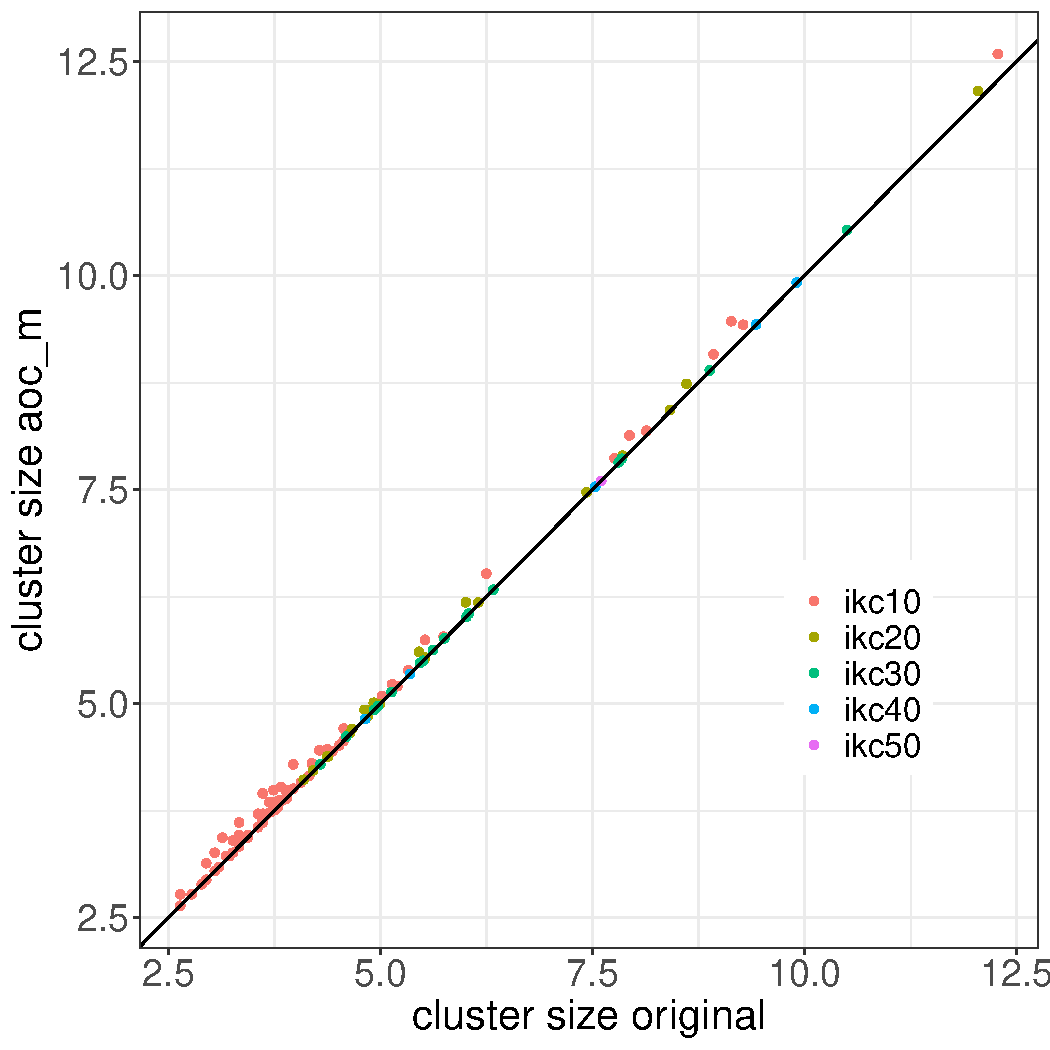
\includegraphics[width=\linewidth]{fig1b.pdf} 
	 \end{subfigure}
 \hfill
	\begin{subfigure}[t]{0.48\textwidth}
        \centering
        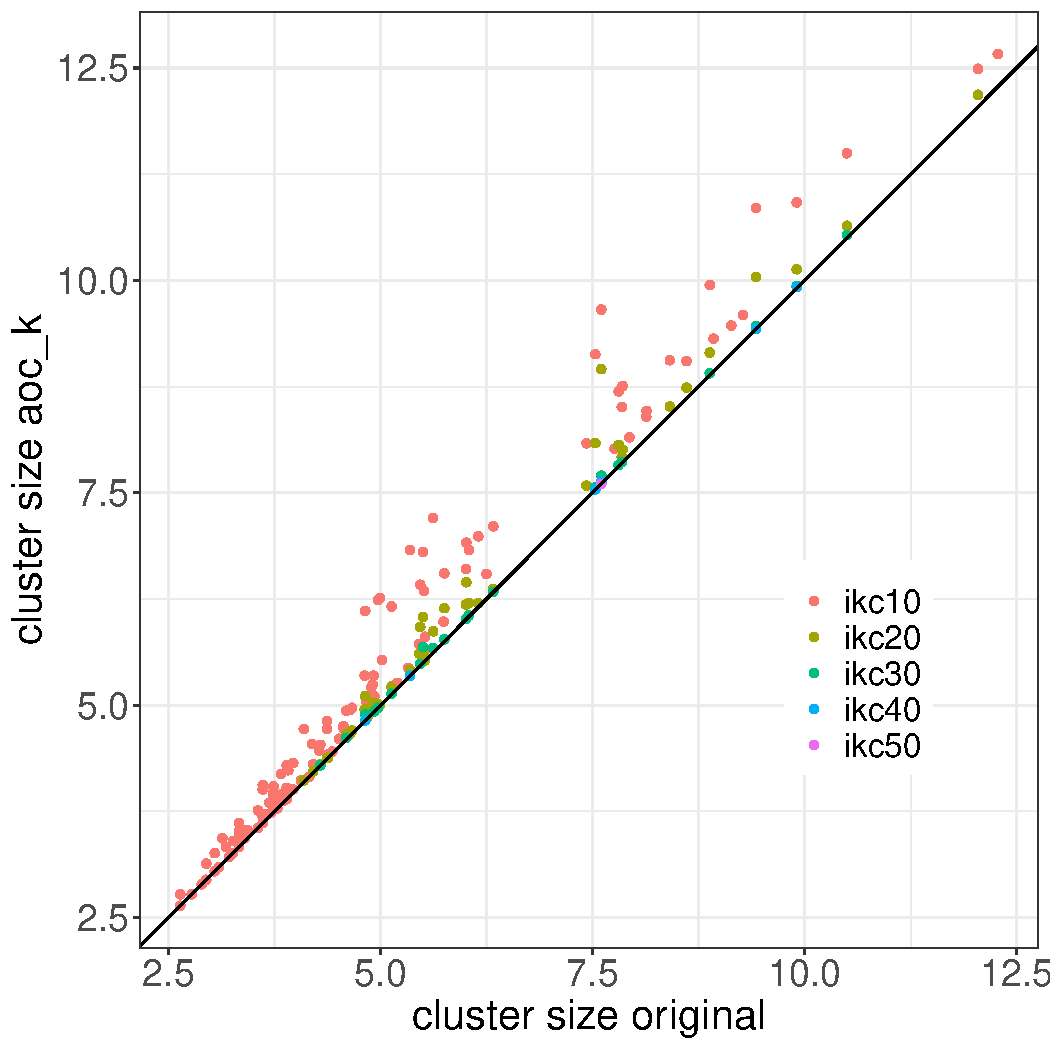
\includegraphics[width=\linewidth]{fig1a.pdf} 
        	\end{subfigure}
\captionsetup{width=0.9\textwidth}	
\caption{Comparison of cluster sizes between disjoint (IKC)  and overlapping (AOC) clusters. Clusters were generated from the CEN network by IKC using values of $k$ ranging from 10 to 50. These clusters were then enriched through the AOC process enforcing either \emph{mcd} (left panel) or \emph{k} (right panel). The input to AOC was the  clustering produced by 
IKC, the value $k$ used to construct the clustering, and the set of nodes to be distributed to additional clusters was all the nodes in the IKC clusters.  Points that lie on the diagonal indicate no change in cluster size after AOC treatment. A natural log scale is used for both axes.}
\label{fig:fig1}
\end{figure}

\begin{table}[H]
\centering
\begin{tabular}{rlcc}
  \hline
 & AOC\_m & \# clusters that do not change & \# clusters that increase\\ 
  \hline
1 & ikc10 &  33 &  95 \\ 
2 & ikc20 &  10 &  34 \\ 
3 & ikc30 &   8 &  14 \\ 
4 & ikc40 &   3 &   3 \\ 
5 & ikc50 &   1 &   0 \\ 
   \hline
\end{tabular}
\quad
\begin{tabular}{rlcc}
  \hline
 & AOC\_k& \# clusters that do not change & \# clusters that increase \\ 
  \hline
1 & ikc10 &  17 & 111 \\ 
2 & ikc20 &   2 &  42 \\ 
3 & ikc30 &   4 &  18 \\ 
4 & ikc40 &   2 &   4 \\ 
5 & ikc50 &   1 &   0 \\ 
   \hline
\end{tabular}
\captionsetup{width=0.9\textwidth}
\caption{Count of IKC clusters that do not change or increase in size, after AOC\_m or AOC\_k treatment of IKC clustering for various values of $k$. For $k=50$, IKC returns a single cluster, at at $k=10$, 128 clusters result.}
\label{tab:tab2}
\end{table}

We then examined the distribution of clusters per candidate node after AOC treatment of clusterings generated by  IKC. For AOC\_k treatment of IKC\_k10 clusters, 54\% of nodes in non-singleton clusters were assigned to between 2 and 24 clusters in a progressively decreasing manner with roughly 26\% of nodes assigned to 2 clusters and a single node being assigned to 24 different clusters (Table~\ref{tab:tab3}). 
The remaining 46\% of the nodes were assigned to a single cluster. 
AOC\_m, in comparison to AOC\_k, results in fewer multiple cluster assignments because of its more stringent membership criterion (Table~\ref{tab:tab2} and Figure~\ref{fig:fig2}).

\begin{figure}[H]
	\centering
	\begin{subfigure}[t]{0.48\textwidth}
	 \centering
	 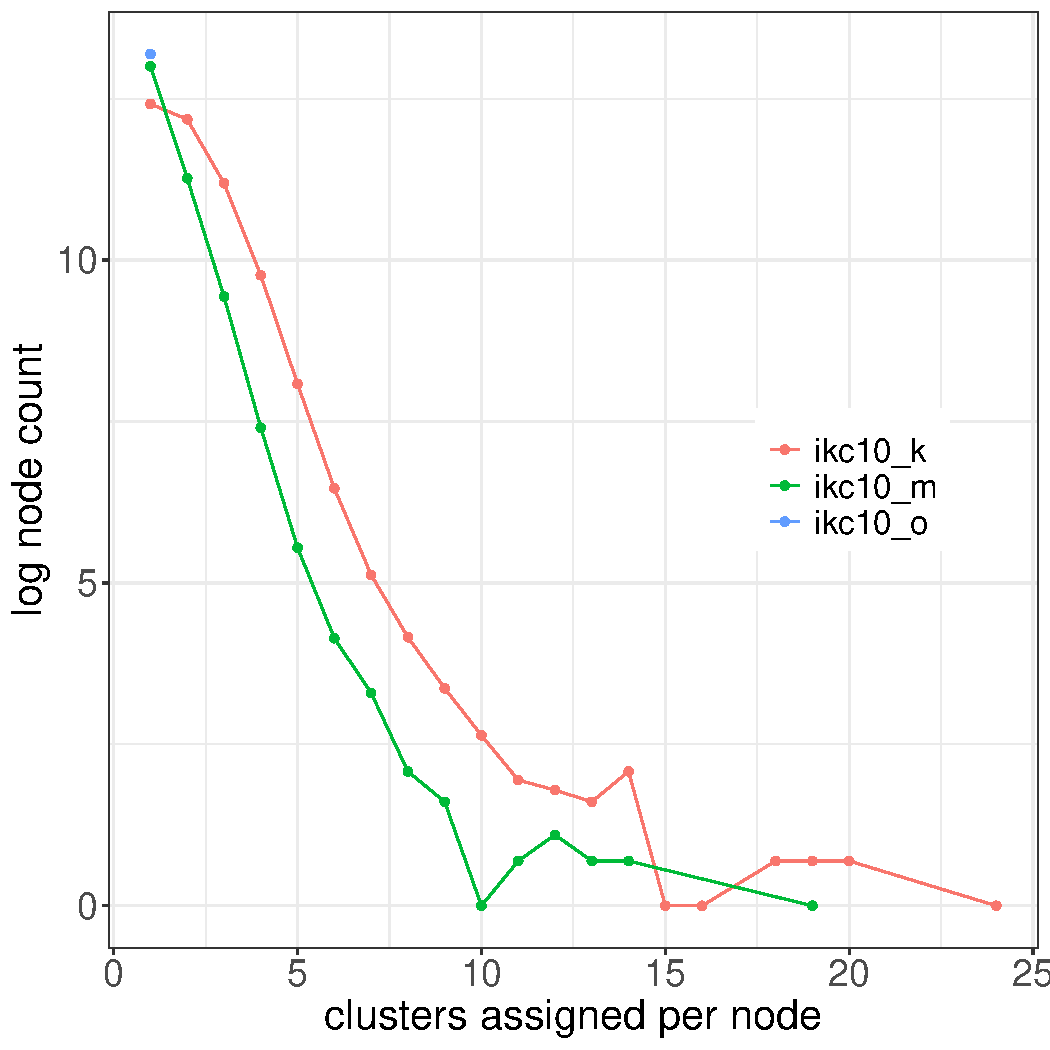
\includegraphics[width=\linewidth]{fig2a.pdf} 
	 \end{subfigure}
 \hfill
	\begin{subfigure}[t]{0.48\textwidth}
        \centering
        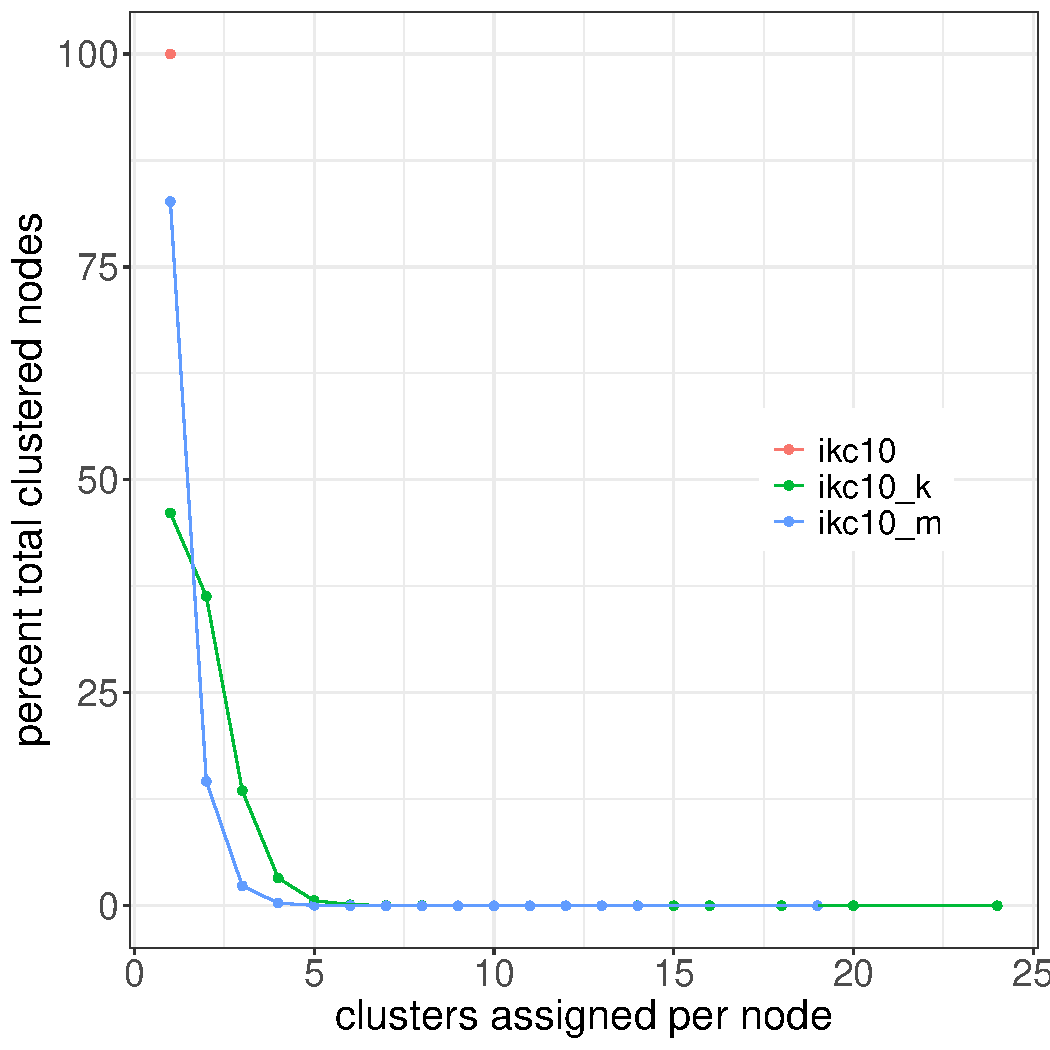
\includegraphics[width=\linewidth]{fig2b.pdf} 
    	\end{subfigure}
\captionsetup{width=0.9\textwidth}	
\caption{AOC selectively assigns nodes to multiple clusters. The figure shows the count of nodes plotted against how many clusters a node was assigned to after AOC treatment enforcing either \emph{k} (ikc10\_k, red) or \emph{mcd} (ikc10\_m, green);  these are shown as natural log counts (left panel) or percentages of the number of nodes (right panel) in non-singleton clusters. One node is assigned to 24 different clusters in the case of AOC\_k. The single blue point in both plots (top left) indicates that all the nodes in the input IKC\_k10 clustering are in single clusters. NEED TO CHANGE ikc10\_o to ikc10.}
\label{fig:fig2}
\end{figure}

\subsection{Which node properties impact multiple assignments?}

To ask whether node degree is associated with the number of clusters assigned to, we examined the 535,165 nodes in non-singleton clusters  from IKC\_k10 clustering of the CEN, and compared their total in-graph degree to the number of clusters they were assigned, after either in AOC\_m or AOC\_k treatments (Figure~\ref{fig:fig3}). 

We partitioned the nodes into five groups based on their total in-network degree (in\_degree + out\_degree),  with group 1 containing the nodes with the smallest total degree (less than 100), group 2 the nodes with total degree between 100 and 999, group 3 the nodes with total degree between 1000 and 9,999, 
group 4 the nodes with total degree between 10,000 and 99,999, and group 5 the nodes with total degree at least 100,000.
Although group classification is based on total degree, no publication has more than 250 references so any publication with high total 
in-network degree by necessity also has high  in-network citation count. 

Of these 535,165 nodes, 50.9\% are  in group 1, 47.6\% are in group  2, 1.5\% are in group 3,  0.03\% are in group 4, and 0.0007\% are in group 5.
Thus, 98.5\% are in groups 1 and 2 with total degree less than 100. Membership in group 3  reflects a high citation count, and membership
in groups 4 or 5 (the top 169 nodes by total degree represents nodes with very high citation counts (degree greater than 1,000 and as high as 256,xxx).

We first compare clusterings produced by AOC\_m and AOC\_k (left subfigure), which shows that the number of clusters assignments per node is larger for AOC\_k than for AOC\_m. This is not unexpected since AOC\_m is a more stringent membership criterion. 
For both AOC\_m and AOC\_k, the number of clusters that any node is assigned to increases as we move from group 1 to group 5, showing
that in general total degree is correlated with the number of clusters that a node is assigned to.
Hence, in-network citation count is associated with the number of clusters that a publication is a core member of.

However, the distributions for each group overlap, revealing potentially interesting differences between publications that are not
explained by citation count alone. Here we discuss these differences, specifically in the context of AOC\_k. 
The largest number of clusters any node is assigned to is 24 and the smallest number is 1. However, all the nodes assigned to 14 or more communities are in groups 4 or 5, 
and so have total degree at least 10,000. Thus,  only the nodes with very high citation counts become members of 14 communities or more. In addition, group 5 publications belong to a minimum of 14 clusters.  
In contrast, every other group has publications that belong to only 1 cluster.  The largest number of communities for publications in groups 1 and 2 is  9, group 3 publications appear in at most 13 communities, 
group 4 publications appear in up to 20 communities, and group 5 publications appear in up to 25 communities.  Since only group 5 publications appear in more than 20 communities, for this network, a very high in-graph citation count is  necessary  for a publication to be assigned to a large number of communities.

While the association between the degree of a node and the likelihood of it being assigned to multiple clusters is evident, there are instances of nodes of relatively low degree being assigned to multiple clusters and nodes of relatively high degree being assigned to one or two clusters. Examining small numbers of such cases did not reveal any obvious qualities that would explain this pattern. This underscores the case for mixed methods approaches to understand how to interpret publication influence and roles within communities and the overall network, given these patterns. This shows that  the number of communities a publication belongs to, although influenced by its total degree (and hence by its citation count), provides an additional perspective into the publication, especially since having a very large total degree (above 10,000) is not sufficient  for membership in many communities. \textcolor{red}{The last three paragraphs are repetitive. I also want @Srijan to comment.}

\begin{figure}[H]
% generated by fig_tier_cluster_counts_3.R 
\centering
	\begin{subfigure}[t]{0.48\textwidth}
	 \centering
	 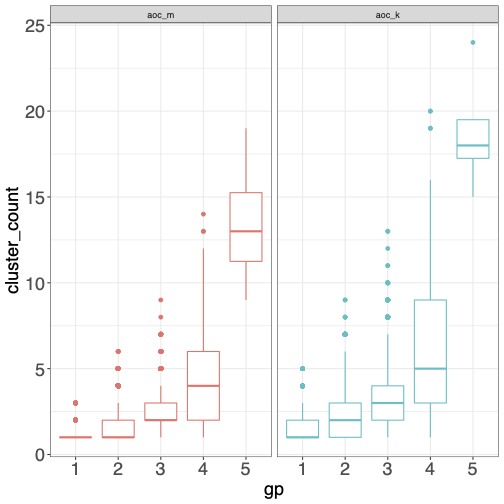
\includegraphics[width=\linewidth]{cluster_group.png} 
	 \end{subfigure}5
 \hfill
	\begin{subfigure}[t]{0.48\textwidth}
        \centering
        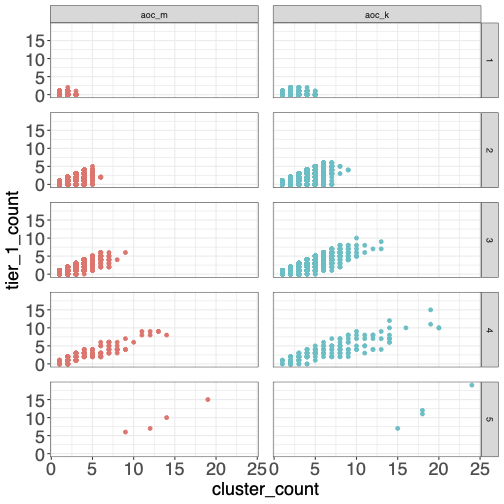
\includegraphics[width=\linewidth]{tier_cluster.png} 
    	\end{subfigure}
\captionsetup{width=0.9\textwidth}	
\caption{Cluster and tier assignments by node degree. The subfigure on the left shows the distribution of numbers of clusters each publication belongs to, and the subfigure on the right shows cluster count by Tier 1 membership for each group; each subfigure presents these results for both AOC\_m and AOC\_k. Nodes are partitioned into five groups based on their total in-network degree (in\_degree + out\_degree) with group 1 containing the nodes with the smallest total degree and group 5 with the nodes with the largest total degree. Group 1 has the largest number of observations and group 5 has the smallest. Group statistics (gp no; class limit; no of nodes): [gp1; $<$100;  272,395], [gp2; 100-999; 254,832], [gp3; 1,000-9,999; 7,773], [gp4; 10,000-99,999; 161], and [gp5; $\geq$100,000; 4]. }
\label{fig:fig3}
\end{figure}

Another perspective that provides additional insight into publications is local influence, their ``tier" within their communities. In \cite{Chandrasekharan2021}, we  proposed a tier classification for nodes in a cluster, in which Tier 1 refers to the nodes in the top 10th percentile with respect to intra-cluster citations. In other words, when measuring in-degree within the cluster, a Tier 1 node is in the top 10 percent compared to all other nodes in its cluster. here we consider Tier 1 profiles within the different communities for each publication .
 
We observe that nodes assigned to multiple clusters are more likely to have Tier 1 status (Figure~\ref{fig:fig3}, right subfigure). The Tier 1 count increases for AOC\_k compared to AOC\_m; since cluster size  increases for AOC\_k compared to AOC\_m and Tier 1 contains the top 10\% of the nodes in each cluster, this is also as expected. \textcolor{red}{Let's discuss this last sentence.}

\textcolor{blue}{George, do we want to provide more information than this scatterplot. Actually I think it would be good to specifically discuss these four papers in Group 5?}


These trends show that while total degree is correlated with the number of clusters a publication belongs to and how many clusters it is Tier 1 for,
these values are not determined just by total degree. Thus, the cluster membership and Tier status within their communities provides complementary insights into  the publications that goes beyond its citation count.
  
\subsection{High Degree Singleton Nodes} 
 
IKC clustering of the CEN results in 3.8\% of its nodes being assigned to non-singleton clusters (coverage). A much larger number of nodes (96.3 \%) is assigned to singleton clusters, essentially left unclustered, some of which are highly cited within the CEN. We examine here whether high-degree members of this population can be incorporated into cores after AOC treatment of IKC clusters. 

In the case of the CEN clustered by IKC\_k10, 15,039 nodes in the top 1\% (by degree) of nodes in the network are assigned to singleton clusters.  With AOC\_m using the 15,039 nodes as candidates no additional assignments are made; the output of AOC\_m is indistinguishable from that of IKC\_k10. 

With AOC\_k, however, 7,459 of 15,039 (49.6 \%) of the singleton nodes are now assigned to IKC\_k10 clusters. Most nodes of singleton origin are assigned to only one cluster, and only one node is assigned to 5 clusters (Figure~\ref{fig:singleton}). The extent of multiple cluster assignments for these 7,459 nodes is less compared to redistribution of clustered nodes (Table~\ref{tab:tab3}). 

In terms of cluster size increases, this result is also mild in effect; 71\% of the 128 clusters in this AOC\_k treatment do not increase in size. In comparison, 74\% and 87\% of the 128 clusters increase in size with AOC\_m and AOC\_k treatment of 128 IKC clusters with non-singleton nodes as input. 

These observations on reducing the singleton fraction suggest that the recursive disjoint steps in IKC exclude nodes that would otherwise qualify for inclusion in cores. We qualitatively examined a small sample of twenty five publications (Supplementary Materials) from the 7,459 singletons that were assigned to IKC clusters in this experiment. The top 25 by indegree largely concerned areas of research such as information theory and decision theory (Supplementary Materials) suggesting relevance through weak ties \citep{granovetter1973strength} or marginally relevant publications. Further study will be necessary to resolve this question of useful discovery but the experiment demonstrates that recycling singletons back into clusters is a feasible user option and has value from the perspective of increasing coverage. 

\begin{figure}[H]
	\centering
	 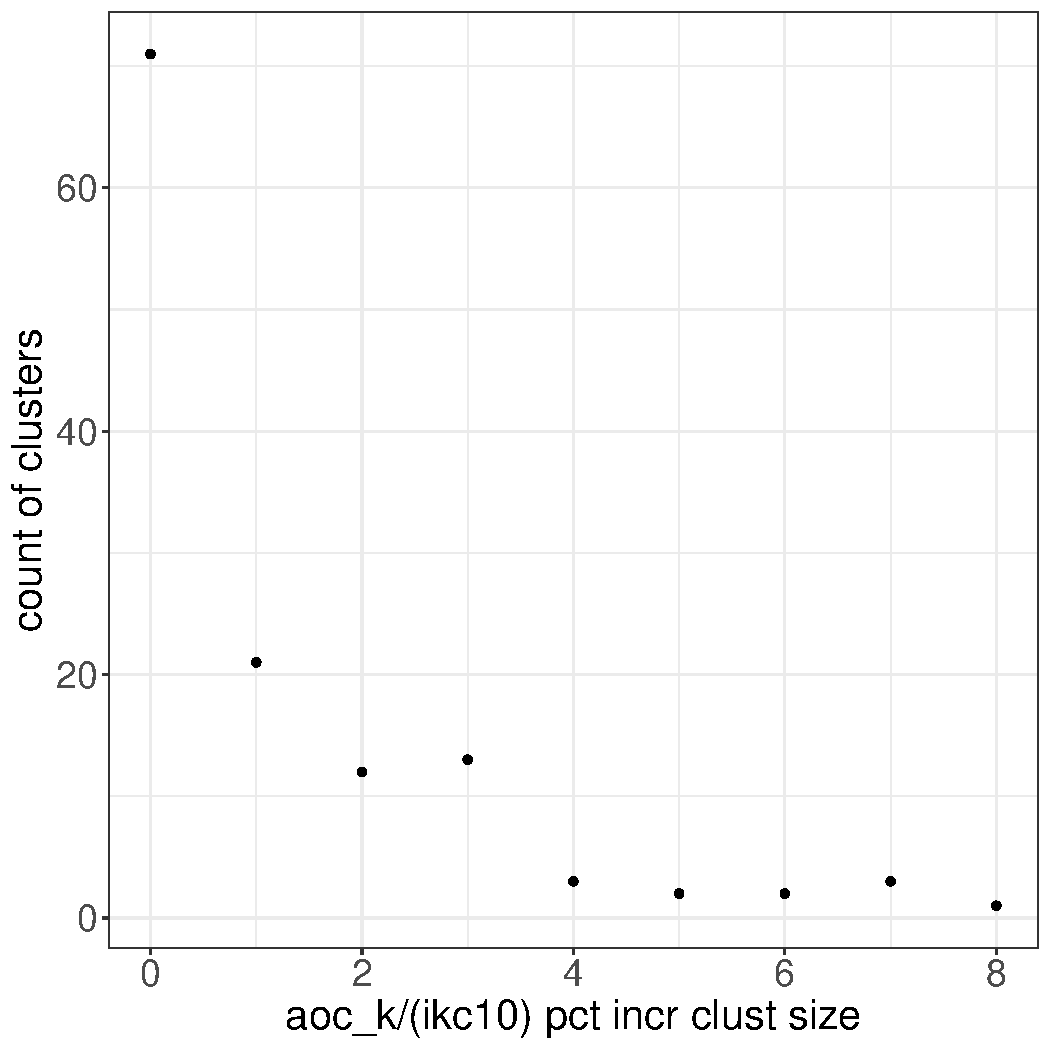
\includegraphics[width=0.6\linewidth]{singletons.pdf} 
\captionsetup{width=0.9\textwidth}
\caption{AOC\_k but not AOC\_m incorporates high-degree singleton nodes from IKC\_k10 into clusters. 15,039 nodes belonging to the top  1\% of nodes by total degree in the CEN were assigned to singleton clusters after IKC\_k10 clustering. 
These 15,039  nodes were used as candidate nodes for AOC\_m and AOC\_k treatment of IKC\_k10 clusters. After AOC\_m treatment, none of these 15,039 nodes were incorporated into any of the 128 clusters resulting from  IKC\_k10. After the more permissive AOC\_k protocol, 7,459 (49.6\%) were incorporated into one or more of the 128 IKC\_k10 clusters. The count of clusters is plotted against percent increase in cluster size for all 128 clusters. The maximum increase in cluster size was 8\%. The majority of the clusters (71\%) did not change in size. After AOC\_k treatment, 540,883 nodes (99\%) of the nodes were assigned to one cluster, 1504 to 2 clusters, 210 to 3 clusters, and 26 to 4 clusters. One node was assigned to 5 clusters.}
\label{fig:singleton}
\end{figure}

\subsection{Marker node distributions}

The SABPQ protocol  \citep{Wedell2022} used to construct the CEN is inclusive by design. It captures nodes that are proximal, by citation, to a seed set identified through a lexical search. The number of nodes in the CEN is roughly two orders of magnitude larger than the nodes in the seed set. The distribution of clusters resulting from the application of one method or another is of interest from a graph theoretic perspective. However, from the perspective of discovery, we are specifically interested in those communities pertinent to EV biology. Therefore, we used 1,021 marker nodes (Materials and Methods) to identify those communities rich in EV content. 

All 1021 markers were found in non-singleton clusters after IC\_k10, AOC\_m, or AOC\_k. Of 128 IKC clusters, 17 contained marker nodes. Three of these 17 clusters (cluster numbers 3, 4 and 35) contained 167, 416, and 310 markers respectively and accounted for 87.5\% of 1021 markers. These clusters exhibited size and MCD as follows. Cluster 3 (170413, 26), Cluster 4 (214877, 14), Cluster 20 (5478, 20), Cluster 25 (1869, 49). 

With both AOC\_m and AOC\_k the concentration of markers increased compared to IKC (Figure~\ref{fig:marker-node-concentration}) from 1021 (IKC) to 1946 (AOC\_m) and 3220 (AOC\_k) respectively.

In the case of AOC\_m, 20 clusters contained makers with cluster numbers 3,4 and 25 containing 434, 951, and 310 markers. For AOC\_k, 31 clusters contained markers with cluster numbers 3, 4, and 35 containing 733, 966, and 710 markers. In addition, cluster 20 increased its marker count from 18 (IKC) to 20 (AOC\_m) to 152 (AOC\_k). Notably, the proportion of 1021 marker nodes in the network increases from 40.7\% in cluster 4 (r1,c4) of IKC clustering to 93.1\% after AOC m to 94.6\% after AOC k. 

We interpret these observations as a more natural clustering of documents once the restrictions of the EV literature in our network once disjoint clustering are lifted. In particular, clusters 3, 4, 20, and 35 merit qualitative examination as communities of EV research on account of their high marker node counts. It should be noted (Table~\ref{tab:marker-node-table}) that clusters 3 and 4 are large ($>$ 100,000 nodes) :whereas clusters 20 and 25 are relatively small ($<$ 10,000 nodes). \textcolor{red}{note to Srijan to critique}

\begin{figure}[H]
% generated from spring_2022_research/george/marker_heatmap.R
	\centering
	 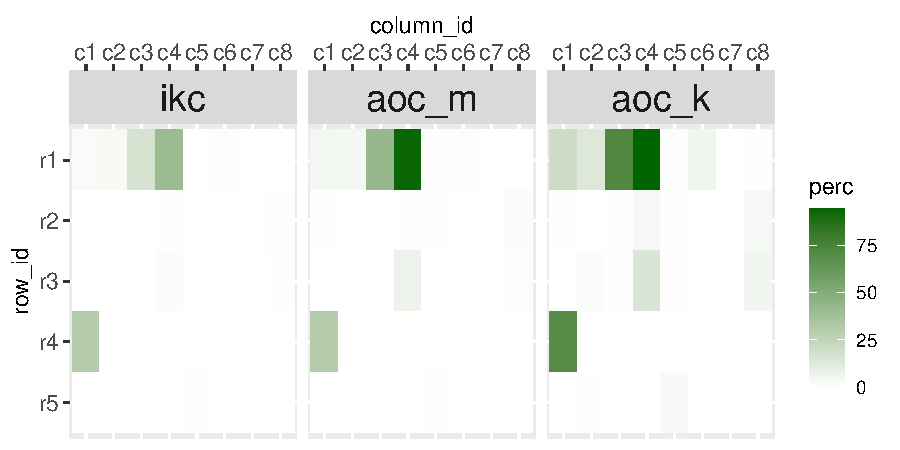
\includegraphics[width=0.9\linewidth]{marker_comps_wide.pdf} 
\captionsetup{width=0.9\textwidth}
\caption{AOC\_m and AOC\_k increase marker node concentrations in IKC clusters. Data are shown for the 40 of 128 IKC clusters with non-zero marker node counts in IKC.  We show marker node counts in 40 clusters (shown in 5 rows with 8 clusters per row) before and after AOC.  Notably, the proportion of 1021 marker nodes in the network increases from 40.7\% in cluster 4 (r1,c4) of IKC clustering to 93.1\% after AOC\_m to 94.6\% after AOC\_k. The proportion of markers in cluster 25 (r4,c1) is the same for IKC and AOC\_m but increases to  69.5\% under the more permissive conditions of AOC\_k. Data for all 128 clusters are available in Supplementary Material.}
\label{fig:marker-node-concentration}
\end{figure}

\clearpage

%xtable(marker_suppl_data[aoc_k_mcount >0 ])
% latex table generated in R 4.2.0 by xtable 1.8-4 package
% Thu Jul 21 12:47:19 2022
\begin{table}[!ht]
\centering
\resizebox{0.9\textwidth}{!}{
\begin{tabular}{ccccccc}
  \hline
cluster\_number & ikc\_mcount & ikc\_size & aoc\_m\_mcount & aoc\_m\_size & aoc\_k\_mcount & aoc\_k\_size \\ 
  \hline
1 &  24 & 36305 &  49 & 37469 & 211 & 98219 \\ 
2 &  39 & 12451 &  44 & 12463 & 140 & 51553 \\ 
{\textbf 3} & 167 & 170413 & 434 & 190427 & 733 & 265681 \\ 
{\textbf 4} & 416 & 214877 & 951 & 293509 & 966 & 316185 \\ 
5 &   1 & 10678 &   5 & 12419 &  14 & 14658 \\ 
6 &   9 & 7207 &   9 & 7284 &  58 & 20893 \\ 
8 &   0 & 3406 &   0 & 3579 &   4 & 4422 \\ 
9 &   2 & 4497 &   3 & 4583 &  12 & 8599 \\ 
10 &   0 & 406 &   0 & 485 &   1 & 736 \\ 
11 &   0 & 1684 &   0 & 1752 &   4 & 3234 \\ 
12 &   3 & 20076 &   6 & 20335 &  40 & 55113 \\ 
13 &   1 & 3419 &   3 & 3597 &   9 & 4731 \\ 
14 &   0 & 124 &   0 & 124 &   1 & 450 \\ 
15 &   0 & 9289 &   2 & 12942 &   2 & 12942 \\ 
16 &  11 & 7528 &  20 & 8790 &  37 & 11093 \\ 
18 &   0 & 2004 &   0 & 2004 &  18 & 15623 \\ 
19 &   0 & 2460 &   0 & 2489 &   3 & 5954 \\ 
 {\textbf {20}} &  18 & 5478 &  76 & 6220 & 152 & 8509 \\ 
21 &   1 & 2553 &   1 & 2595 &   3 & 4961 \\ 
22 &   0 & 408 &   0 & 408 &   2 & 1004 \\ 
23 &   0 & 2343 &   0 & 2606 &   2 & 3035 \\ 
24 &   6 & 2575 &  15 & 2690 &  52 & 6350 \\ 
{\textbf {25}} & 310 & 1869 & 310 & 1871 & 710 & 9241 \\ 
30 &   1 & 470 &   1 & 484 &   1 & 1082 \\ 
34 &   0 & 237 &   0 & 239 &   3 & 612 \\ 
37 &  11 & 276 &  12 & 278 &  28 & 1344 \\ 
50 &   0 & 312 &   0 & 325 &   1 & 396 \\ 
53 &   0 & 561 &   0 & 562 &   1 & 1217 \\ 
66 &   1 & 144 &   1 & 144 &   3 & 512 \\ 
88 &   0 &  39 &   2 &  41 &   2 &  41 \\ 
116 &   0 &  66 &   2 &  74 &   7 &  94 \\ 
   \hline
\end{tabular}}
\captionsetup{width=0.9\textwidth}
\caption{Comparing marker node counts in IKC, AOC\_m, and AOC\_k, The count of markers (mcount) in each IKC cluster as well as the cluster size is shown for any of 128 clusters containing at least one marker node after IKC,  AOC\_m, and AOC\_k treatments. Cluster numbers 3, 4, 20 and 25 contain significantly higher marker counts.}
\label{tab:marker-node-table}
\end{table}

\subsection{Examining overlap between clusters}
Finally, we examine the relationship between AOC modified clusters based on overlap. One way in which the relationship of disjoint clusters to each other can be examined is a normalized count of edges between pairs of clusters \textcolor{red}{Tandy should we invoke Subelj, Shun and intercluster conductance?}. From the perspective of overlapping clusters, however, it is possible to establish similarity by counting the number of nodes in common. Accordingly, we computed overlapping node counts between clusters for either AOC\_m or AOC\_k treatments of IKC10 clusters and normalized these inersectional measures using the Jaccard Coefficient (JC). A threshold of greater than  the median JC was set to allow an edge. The results are visualized in Figure~\ref{fig:overlapping}.

With AOC\_m, five connected components results that contain a total of 20 clusters. The largest contains 8 clusters. With the more permissive AOC\_k protocol, 4 connected components result consisting of 31 clusters, with the largest component consisting of 25 clusters. As we indicate earlier, clusters 23, 20, and 25 are richest in marker nodes and of greatest relevance to EV research. With AOC\_m, clusters 3 and 4 are in a single component and clusters 20 and 25 are in another one. With AOC\_k, all four clusters are in the single large component. Thus, beyond graph theoretic measures of cluster quality such as conductance or modularity, users have the ability to apply either a stringent (AOC\_m) or a permissive (AOC\_k) approach (or perhaps both) to support qualitative interpretation.

A number of future opportunities, accompanied by challenges, are evident. First, a qualitative demonstration that this overlapping approach better captures communities of publications than a comparable disjoint method. Second, a temporal analysis of the growth of communities of interest,  Third, further insight into global (network) versus local (community) influence. 
Fourth, an understanding of the collaboration patterns of authors in these communities. Fifth, identifying influence at the level of the author rather than publication. Sixth, bringing to light, the institutional and financial support that enabled this research. Last...


\begin{figure}[H]
	\centering
	\begin{subfigure}[t]{0.48\textwidth}
	 \centering
	 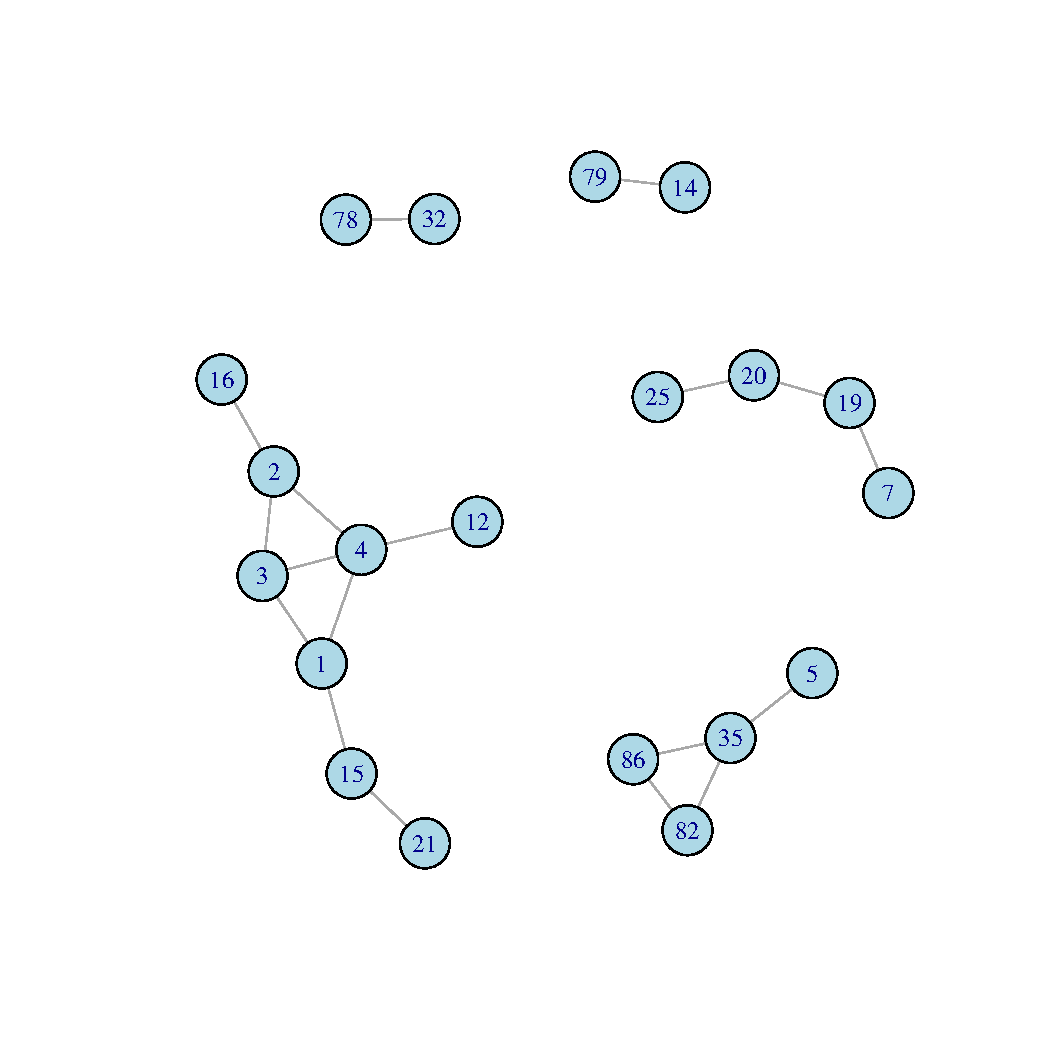
\includegraphics[width=\linewidth]{ikc10_m_pw.pdf} 
	 %\caption{Generic fig2 a caption} \label{fig:2a}
	 \end{subfigure}
 \hfill
	\begin{subfigure}[t]{0.48\textwidth}
        \centering
        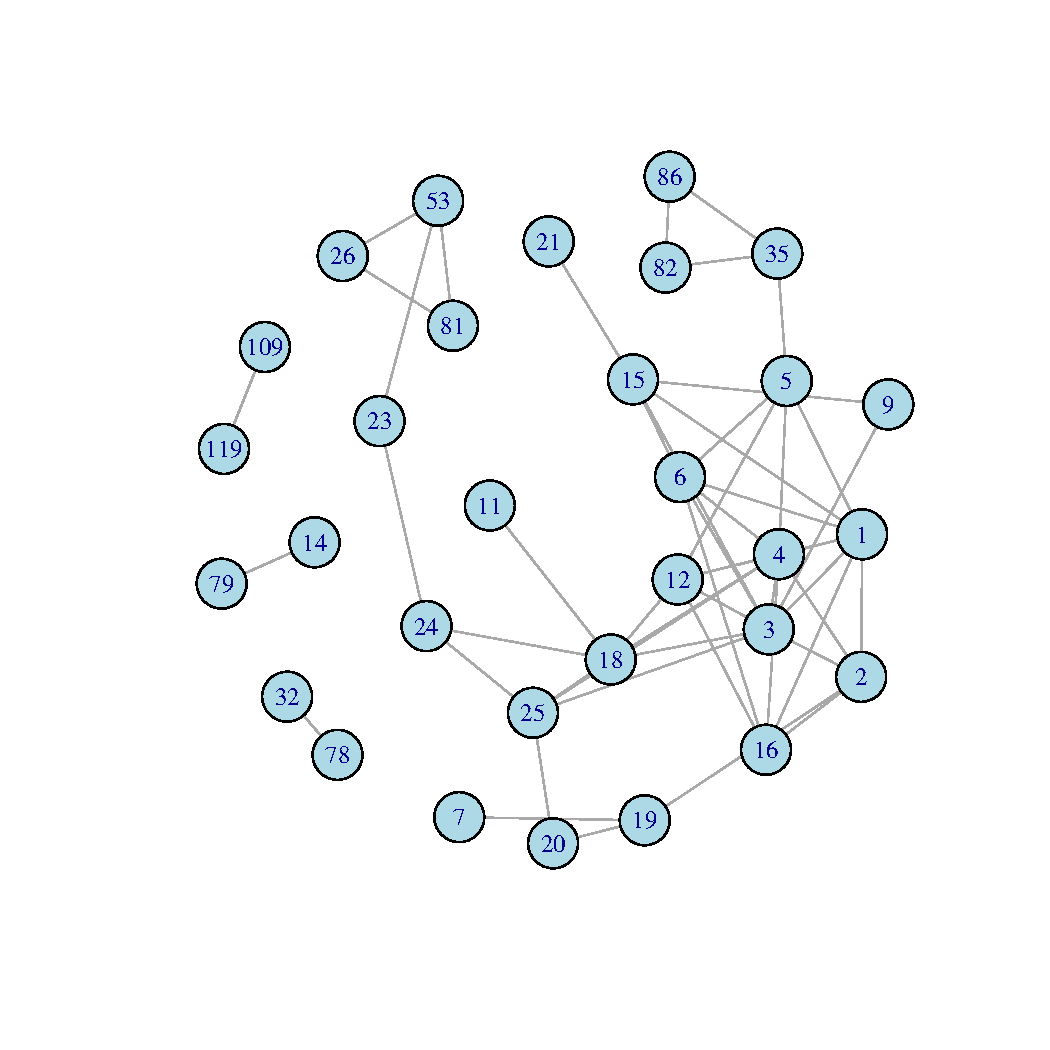
\includegraphics[width=\linewidth]{ikc10_k_pw.pdf} 
        %\caption{Generic fig2 b caption} \label{fig:2b}
    	\end{subfigure}
\caption{Overlapping clusters produced by IKC\_k10 + AOC.  Overlapping clusters were generated from CEN data using IKC\_k10 followed by either AOC\_m (left) or AOC\_k (right). Edges are drawn between clusters based on the Jaccard Coefficient for node overlap and are visible if the JC exceeds the median value. Cluster numbers in both panels correspond to cluster numbers from the input IKC clustering.}
\label{fig:overlapping}
\end{figure}


\clearpage
\begin{sidewaystable}[h!]
\centering
\resizebox{\textwidth}{!}{
\begin{tabular}{clllllllllll}
  \hline
 no\_clusters & ikc10\_k & ikc10\_m & ikc20\_k & ikc20\_m & ikc30\_k & ikc30\_m & ikc40\_k & ikc40\_m & ikc50\_k & ikc50\_m \\ 
  \hline
1 & 246787 & 442485 & 221728 & 254435 & 85515 & 86806 & 36367 & 36463 & 2004 & 2004 \\ 
2 & 194427 & 78150 & 49195 & 20280 & 2731 & 1487 & 363 & 269 &  &  \\ 
3 & 72367 & 12518 & 4511 & 1057 &  82 &  43 &   4 &   2 &  &  \\ 
4 & 17401 & 1642 & 377 &  98 &  15 &   8 &  &  &  &  \\ 
5 & 3232 & 256 &  61 &  21 &   2 &   1 &  &  &  &  \\ 
6 & 641 &  63 &  19 &   5 &  &  &  &  &  &  \\ 
7 & 168 &  27 &   4 &  &  &  &  &  &  &  \\ 
8 &  64 &   8 &   1 &   1 &  &  &  &  &  &  \\ 
9 &  29 &   5 &   1 &  &  &  &  &  &  &  \\ 
10 &  14 &   1 &   1 &   1 &  &  &  &  &  &  \\ 
11 &   7 &   2 &  &  &  &  &  &  &  &  \\ 
12 &   6 &   3 &  &  &  &  &  &  &  &  \\ 
13 &   5 &   2 &  &  &  &  &  &  &  &  \\ 
14 &   8 &   2 &  &  &  &  &  &  &  &  \\ 
15 &   1 &  &  &  &  &  &  &  &  &  \\ 
16 &   1 &  &  &  &  &  &  &  &  &  \\ 
18 &   2 &  &  &  &  &  &  &  &  &  \\ 
19 &   2 &   1 &  &  &  &  &  &  &  &  \\ 
20 &   2 &  &  &  &  &  &  &  &  &  \\ 
24 &   1 &  &  &  &  &  &  &  &  &  \\ 
   \hline
\end{tabular}}
%:
\caption{Cluster Size Increases After AOC Treatment. The count of clusters that either increase in size (increase) or remain the same size (no\_change) is shown for either AOC\_m (left) or AOC\_k (right) treatment for five different values of $k$ and where the nodes allowed to be in multiple clusters are those that appear in one non-singleton cluster in IKC(k). For $k=50$, IKC returns a single cluster, by definition, the cluster does not change after AOC treatment. At at $k=10$, 128 clusters result.}
\label{tab:tab3}
\end{sidewaystable}

\clearpage

\section{Conclusions} The methods and results described in this article speak to a focus on method development for exploratory discovery. One objective is to construct a modular community finding pipeline that is subject-independent and has options for users. A second objective is non-disjoint clustering. A third is community detection in context. Our test case is the EV literature. In combining the two, we have sought to include human experience and intent \citep{vonluxburg2012clustering} through controlling the input data and designing applying contextual evaluation criteria.

Add more..after discussion.


\section*{Competing Interests} \vspace{3mm} The authors have no competing interests. Dimensions data were made available by Digital Science through the \href{http://www.dimensions.ai/scientometric-research/.}{free data access for scientometrics research projects program}. Digital Science personnel did not participate in conceptualization, experimental design, review of results, or conclusions presented. 

\section*{Funding Information} TW receives funding from the Grainger Foundation. Research reported in this manuscript was supported by the Google Cloud Research Credits program through award GCP19980904 to GC.

\section*{Data Availability} Access to the bibliographic data analyzed in this study requires access from Digital Science. Code generated for this study is freely available from our Github site \citep{Park2021}.

\section*{Acknowledgments} We thank Digital Science, Google, and the Grainger Foundation.

\bibliographystyle{apalike}
\bibliography{akhil.bib}
\end{document}
%%%%%%%%%%%%%%%%
%%%%%%%%%%%%%%%%
%%%%%%%%%%%%%%%%
%%%%%%%%%%%%%%%%

For groups 1--4, there are some publications that are Tier 1 in all communities they belong to, some that are never in Tier 1, but the majority are in between. 
However, while the four publications in group 5 are Tier 1 for at least 7 communities, only one is Tier 1 for more than 10 communities. 
Interestingly, there are four publications in Group 4 that are in Tier 1 for at least 10 communities, two that are Tier 1 in more than 10 communities, and one of these is Tier 1 in 15 communities.


% latex table generated in R 4.1.2 by xtable 1.8-4 package
% Tue Jul 12 10:54:57 2022
\begin{table}[ht]
\centering
\begin{tabular}{rrrrr}
  \hline
 & cluster\_id & ikc10 & aoc\_m & aoc\_k \\ 
  \hline
1 &   1 & 36305 & 36305 & 115426 \\ 
  2 &   2 & 12451 & 12451 & 38000 \\ 
  3 &   3 & 170413 & 170413 & 436231 \\ 
  4 &   4 & 214877 & 214877 & 295184 \\ 
  5 &   5 & 10678 & 10678 & 15308 \\ 
  6 &   6 & 7207 & 7207 & 21875 \\ 
  7 &   7 & 2795 & 2795 & 2919 \\ 
  8 &   8 & 3406 & 3406 & 5768 \\ 
  9 &   9 & 4497 & 4497 & 13965 \\ 
  10 &  10 & 406 & 406 & 771 \\ 
  11 &  11 & 1684 & 1684 & 4591 \\ 
  12 &  12 & 20076 & 20076 & 68398 \\ 
  13 &  13 & 3419 & 3419 & 6302 \\ 
  14 &  14 & 124 & 124 & 619 \\ 
  15 &  15 & 9289 & 9289 & 9289 \\ 
  16 &  16 & 7528 & 7528 & 12689 \\ 
  17 &  17 & 206 & 206 & 249 \\ 
  18 &  18 & 2004 & 2004 & 12757 \\ 
  19 &  19 & 2460 & 2460 & 9636 \\ 
  20 &  20 & 5478 & 5478 & 11505 \\ 
  21 &  21 & 2553 & 2553 & 7766 \\ 
  22 &  22 & 408 & 408 & 1327 \\ 
  23 &  23 & 2343 & 2343 & 3743 \\ 
  24 &  24 & 2575 & 2575 & 5966 \\ 
  25 &  25 & 1869 & 1869 & 4982 \\ 
  26 &  26 & 133 & 133 & 420 \\ 
  27 &  27 & 125 & 125 & 228 \\ 
  28 &  28 &  96 &  96 & 134 \\ 
  29 &  29 & 421 & 421 & 1184 \\ 
  30 &  30 & 470 & 470 & 1248 \\ 
  31 &  31 &  40 &  40 &  43 \\ 
  32 &  32 & 517 & 517 & 568 \\ 
  33 &  33 & 135 & 135 & 310 \\ 
  34 &  34 & 237 & 237 & 623 \\ 
  35 &  35 & 210 & 210 & 679 \\ 
  36 &  36 &  84 &  84 & 142 \\ 
  37 &  37 & 276 & 276 & 857 \\ 
  38 &  38 & 250 & 250 & 474 \\ 
  39 &  39 & 251 & 251 & 293 \\ 
  40 &  40 & 248 & 248 & 723 \\ 
  41 &  41 &  79 &  79 & 144 \\ 
  42 &  42 &  38 &  38 &  45 \\ 
  43 &  43 &  80 &  80 & 146 \\ 
  44 &  44 &  49 &  49 &  50 \\ 
  45 &  45 &  37 &  37 &  48 \\ 
  46 &  46 & 234 & 234 & 466 \\ 
  47 &  47 &  47 &  47 &  47 \\ 
  48 &  48 &  99 &  99 & 245 \\ 
  49 &  49 & 103 & 103 & 198 \\ 
  50 &  50 & 312 & 312 & 468 \\ 
  51 &  51 & 181 & 181 & 269 \\ 
  52 &  52 &  28 &  28 &  28 \\ 
  53 &  53 & 561 & 561 & 2177 \\ 
  54 &  54 &  18 &  18 &  18 \\ 
  55 &  55 & 128 & 128 & 312 \\ 
  56 &  56 &  44 &  44 &  54 \\ 
  57 &  57 & 100 & 100 & 100 \\ 
  58 &  58 & 138 & 138 & 307 \\ 
  59 &  59 &  73 &  73 & 218 \\ 
  60 &  60 &  37 &  37 &  37 \\ 
  61 &  61 &  21 &  21 &  23 \\ 
  62 &  62 &  72 &  72 &  72 \\ 
  63 &  63 & 245 & 245 & 1040 \\ 
  64 &  64 &  53 &  53 &  56 \\ 
  65 &  65 &  41 &  41 &  42 \\ 
  66 &  66 & 144 & 144 & 346 \\ 
  67 &  67 &  23 &  23 &  23 \\ 
  68 &  68 & 106 & 106 & 295 \\ 
  69 &  69 & 244 & 244 & 362 \\ 
  70 &  70 &  45 &  45 &  45 \\ 
  71 &  71 &  96 &  96 & 110 \\ 
  72 &  72 &  37 &  37 &  39 \\ 
  73 &  73 &  31 &  31 &  36 \\ 
  74 &  74 & 151 & 151 & 320 \\ 
  75 &  75 &  26 &  26 &  26 \\ 
  76 &  76 & 315 & 315 & 1383 \\ 
  77 &  77 & 147 & 147 & 379 \\ 
  78 &  78 & 169 & 169 & 407 \\ 
  79 &  79 &  46 &  46 &  68 \\ 
  80 &  80 &  49 &  49 &  80 \\ 
  81 &  81 &  42 &  42 &  84 \\ 
  82 &  82 &  79 &  79 & 116 \\ 
  83 &  83 & 123 & 123 & 305 \\ 
  84 &  84 &  31 &  31 &  47 \\ 
  85 &  85 &  26 &  26 &  26 \\ 
  86 &  86 & 137 & 137 & 314 \\ 
  87 &  87 &  43 &  43 &  85 \\ 
  88 &  88 &  39 &  39 &  40 \\ 
  89 &  89 &  53 &  53 &  53 \\ 
  90 &  90 &  60 &  60 & 114 \\ 
  91 &  91 & 170 & 170 & 170 \\ 
  92 &  92 &  80 &  80 & 127 \\ 
  93 &  93 &  19 &  19 &  21 \\ 
  94 &  94 &  42 &  42 &  48 \\ 
  95 &  95 &  58 &  58 &  62 \\ 
  96 &  96 &  49 &  49 &  52 \\ 
  97 &  97 &  28 &  28 &  34 \\ 
  98 &  98 &  67 &  67 & 120 \\ 
  99 &  99 &  28 &  28 &  28 \\ 
  100 & 100 &  35 &  35 &  37 \\ 
  101 & 101 &  16 &  16 &  17 \\ 
  102 & 102 &  42 &  42 &  51 \\ 
  103 & 103 &  14 &  14 &  14 \\ 
  104 & 104 &  45 &  45 &  45 \\ 
  105 & 105 &  37 &  37 &  40 \\ 
  106 & 106 &  64 &  64 &  64 \\ 
  107 & 107 &  91 &  91 & 142 \\ 
  108 & 108 &  14 &  14 &  14 \\ 
  109 & 109 &  30 &  30 &  52 \\ 
  110 & 110 &  28 &  28 &  28 \\ 
  111 & 111 &  46 &  46 &  78 \\ 
  112 & 112 &  49 &  49 &  53 \\ 
  113 & 113 &  22 &  22 &  22 \\ 
  114 & 114 &  37 &  37 &  46 \\ 
  115 & 115 &  24 &  24 &  28 \\ 
  116 & 116 &  66 &  66 &  97 \\ 
  117 & 117 &  50 &  50 &  66 \\ 
  118 & 118 &  25 &  25 &  25 \\ 
  119 & 119 &  35 &  35 &  38 \\ 
  120 & 120 &  18 &  18 &  18 \\ 
  121 & 121 &  19 &  19 &  19 \\ 
  122 & 122 &  28 &  28 &  30 \\ 
  123 & 123 &  30 &  30 &  32 \\ 
  124 & 124 &  21 &  21 &  21 \\ 
  125 & 125 &  37 &  37 &  52 \\ 
  126 & 126 &  28 &  28 &  28 \\ 
  127 & 127 &  21 &  21 &  23 \\ 
  128 & 128 &  28 &  28 &  28 \\ 
   \hline
\end{tabular}
\caption(blah blah blah}
\end{table}


